% chapter15.tex -- Why We Cannot Extend This Algorithm to 1-Connected Graphs
% Based on the author's UGThesis.docx.

\chapter{Why We Cannot Extend This Algorithm to 1-Connected Graphs}
\label{ch:one_connected}

In this chapter we discuss the limitations of our algorithm when applied to 1-connected (i.e., connected but not biconnected) plane graphs. 
We show that the existence of separation vertices (cut vertices) leads to faces that contain a vertex multiple times, which can prevent the existence of a safe root. 
Consequently, our algorithm cannot be directly extended to all 1-connected graphs, although it works for a subclass.

\section{Structure of 1-Connected Graphs}
\label{sec:one_connected_structure}

A graph is \textbf{1-connected} (or simply connected) if it has at least one separation vertex (cut vertex). 
Removing a separation vertex disconnects the graph into two or more components. 
In a plane embedding, a separation vertex appears on the boundary of several faces, and a single face may contain the same vertex more than once when traversing its boundary.

This phenomenon is the key obstacle: a face in a 1-connected graph can be a closed walk that visits a vertex multiple times, rather than a simple cycle. 
Our algorithm assumes that each face is a simple cycle (no repeated vertices). 
When a vertex repeats, the face is no longer a simple polygon, and the definition of triangulation becomes ambiguous (multiple copies of the same vertex). 
Moreover, the safe root existence proof (Theorem~\ref{thm:safe_root_exists}) relies on the face being a simple cycle.

\section{Multiple Occurrences of the Same Vertex in a Face}
\label{sec:multiple_occurrences}

Consider the simplest 1-connected graph: a path of four vertices \(1-2-3-4\) (Figure~\ref{fig:path4}). 
This graph is not biconnected because removing vertex 2 or 3 disconnects it. 
When we consider the outer face of this path (embedding it in the plane with edges as straight line segments), the boundary of the outer face is the closed walk
\[
1 \to 2 \to 3 \to 4 \to 3 \to 2 \to 1.
\]
This walk contains vertices 2 and 3 twice each. 
If we try to interpret this walk as a cycle for triangulation, we have a “cycle” with repeated vertices, which is not a simple cycle.

\begin{figure}[htbp]
    \centering
    \begin{tikzpicture}[scale=1.2, every node/.style={circle, draw, fill=white, inner sep=2pt}]
        \node (v1) at (0,0) {1};
        \node (v2) at (2,0) {2};
        \node (v3) at (4,0) {3};
        \node (v4) at (6,0) {4};
        \draw (v1)--(v2)--(v3)--(v4);
        \draw[red, dashed, bend left=45] (v4) to (v3);
        \draw[red, dashed, bend left=45] (v3) to (v2);
        \draw[red, dashed, bend left=45] (v2) to (v1);
        \node at (3, -0.8) {Path graph \(1-2-3-4\)};
        \node at (3, -1.5) {Outer face boundary: \(1-2-3-4-3-2-1\)};
    \end{tikzpicture}
    \caption{A path graph with four vertices. The outer face boundary visits vertices 2 and 3 twice.}
    \label{fig:path4}
\end{figure}

\section{Impossibility of a Safe Root in Such Faces}
\label{sec:no_safe_root_1connected}

Suppose we attempt to apply our algorithm to this face, treating it as a cycle with vertices in the order \(1,2,3,4,3,2,1\) (six distinct positions, but only four distinct vertex labels). 
We would need to choose a safe root vertex from among the distinct vertices (1,2,3,4). 
We examine each candidate:

\begin{itemize}
    \item \textbf{Vertex 1:} Its neighbours on the “cycle” are 2 (first occurrence) and the final 1? Actually, in the walk, vertex 1 appears only at the beginning and end (as the same vertex). 
    The non-neighbouring vertices in the cyclic order are the two copies of 3 and the copy of 4? However, any chord from 1 to a non-neighbour would create a multi-edge because there are already edges incident to the copies. 
    More concretely, the chord \((1,3)\) would duplicate an existing edge? Not exactly, but the problem is that the face is not a simple cycle, so our definition of “chord” and “triangulation” is not well-defined. 
    In practice, one cannot triangulate such a face without creating degenerate triangles or multi-edges.
    
    \item \textbf{Vertex 2:} Appears twice. 
    A chord from 2 to itself would be a loop, which is not allowed. 
    Any chord from one occurrence of 2 to a vertex between the two occurrences would cross the boundary or create a multi-edge.
    
    \item \textbf{Vertex 3:} Similar problems as vertex 2.
    
    \item \textbf{Vertex 4:} Its neighbours are 3 (first occurrence) and the second 3? Actually, in the walk, 4 appears only once, between the two 3’s. 
    Trying to add chords from 4 to non-neighbours (like 1 or the second 2) would either cross the boundary or duplicate existing edges.
\end{itemize}

In fact, no vertex can serve as a safe root because any fan triangulation would either create a loop (if the root appears twice) or a multi-edge with an existing boundary edge. 
Thus our algorithm cannot even initialise a local genealogical tree for this face.

\section{A Counterexample Where the Algorithm Still Works}
\label{sec:counterexample_works}

Not all 1-connected graphs are impossible. 
Consider the graph with vertices \(1,2,3,4,5\) and edges forming the cycle \(1-2-3-4-5-2-1\) (a “lollipop” shape). 
The outer face boundary is \(1-2-3-4-5-2-1\), which still repeats vertex 2. 
However, in this case vertex 1 appears only once, and its neighbours on the boundary are 2 (first) and the final 1? Actually the boundary is \(1 \to 2 \to 3 \to 4 \to 5 \to 2 \to 1\). 
Vertex 1 is adjacent to the first 2 and the last 1? The last vertex is also 1, so it is a loop? Wait, careful: The boundary walk starts at 1, goes to 2, then 3,4,5, then back to 2, then returns to 1. 
So vertex 1 appears only at the start and end (same vertex), so it is a single occurrence. 
Vertex 2 appears twice.

If we choose vertex 1 as the root, its non-neighbouring vertices on the walk are 3,4,5 (since 2 is a neighbour). 
The chords \((1,3)\), \((1,4)\), \((1,5)\) are all valid and do not conflict with any existing edge. 
Thus vertex 1 is a safe root. 
Similarly, vertices 3 and 5 may also be safe. 
Therefore, for this graph, our algorithm can be applied and will generate all valid triangulations.

\begin{figure}[htbp]
    \centering
    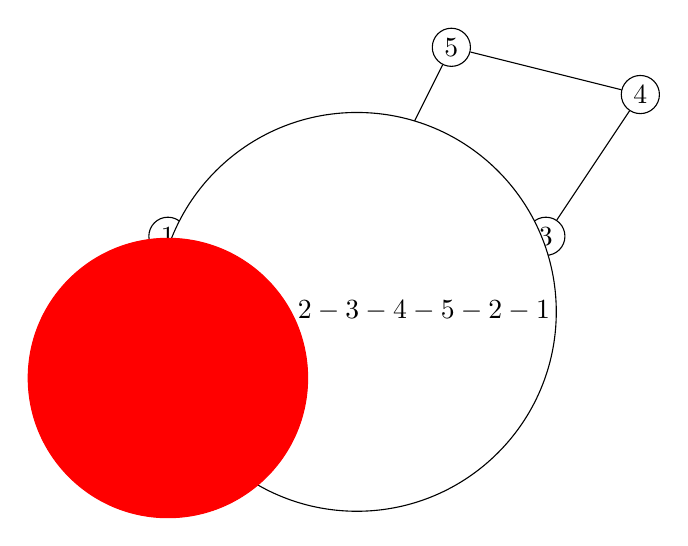
\begin{tikzpicture}[scale=1.2, every node/.style={circle, draw, fill=white, inner sep=2pt}]
        \node (v1) at (0,0) {1};
        \node (v2) at (2,0) {2};
        \node (v3) at (4,0) {3};
        \node (v4) at (5,1.5) {4};
        \node (v5) at (3,2) {5};
        \draw (v1)--(v2)--(v3)--(v4)--(v5)--(v2);
        \draw (v2)--(v1);
        \node at (2, -0.8) {Graph \(1-2-3-4-5-2-1\)};
        \node[red] at (0, -1.5) {Vertex 1 is a safe root};
    \end{tikzpicture}
    \caption{A 1-connected graph where a safe root exists (vertex 1). 
    The outer face boundary is \(1-2-3-4-5-2-1\); vertex 1 appears only once.}
    \label{fig:lollipop}
\end{figure}

\section{Fundamental Limitation}
\label{sec:fundamental_limitation}

The necessary condition for our algorithm to work on a face is that the face boundary is a simple cycle (no repeated vertices) or, if repeated vertices occur, there must be at least one vertex that appears exactly once and whose incident edges do not create conflicts. 
In general 1-connected graphs, faces can have repeated vertices, and it is not guaranteed that such a safe root exists. 
In fact, for the path graph of four vertices, no safe root exists. 
Therefore our algorithm cannot be extended to all 1-connected plane graphs without significant modifications.

\section{Why the Multi-Edge Problem Is Not the Only Issue}
\label{sec:other_issues}

One might think that the multi-edge problem is the only obstacle, and that if we could handle multi-edges, 1-connected graphs would be easy. 
However, the deeper issue is that the very notion of triangulating a face that is not a simple cycle is ambiguous. 
A face with repeated vertices corresponds to a situation where the graph has a cut vertex, and the “inside” of the face is not well-defined as a simple polygon. 
Our algorithm relies on the fact that each face is a simple cycle, which holds for biconnected graphs but fails for 1-connected graphs.

\section{Conclusion}
\label{sec:one_connected_conclusion}

We have shown that our algorithm cannot be directly applied to all 1-connected plane graphs because:
\begin{enumerate}
    \item Faces may contain the same vertex multiple times, violating the simple cycle assumption.
    \item Safe root vertices may not exist (e.g., the path graph of four vertices).
    \item Triangulating such faces is not well-defined in the usual combinatorial sense.
\end{enumerate}
Nevertheless, for certain 1-connected graphs where at least one vertex appears only once on each face boundary and satisfies the safe root condition, our algorithm can still be used. 
A complete extension to 1-connected graphs would require a more fundamental rethinking of face triangulation in the presence of cut vertices, which we leave as future work (Chapter~\ref{ch:future_work}).